\documentclass[12pt,a4paper]{article}
\usepackage[utf8]{inputenc}
\usepackage[T1]{fontenc}
\usepackage[spanish]{babel}
\usepackage{geometry}
\geometry{margin=2.5cm}
\usepackage{graphicx}
\usepackage{booktabs}
\usepackage{tabularx}
\usepackage{longtable}
\usepackage{array}
\usepackage{float}
\usepackage{enumitem}
\usepackage{cite}
\usepackage{microtype}
\usepackage{adjustbox}
\emergencystretch=2em
\usepackage[hidelinks]{hyperref}

\begin{document}

\begin{titlepage}
    \centering
    {\Large \textbf{UNIVERSIDAD T{\'E}CNICA ESTATAL DE QUEVEDO}}\\[0.3cm]
    {\large Facultad de Ciencias de la Computaci{\'o}n}\\
    {\large Carrera de Ingenier{\'i}a en Software}\\[1.5cm]
    {\large \textbf{Asignatura:} Ingenier{\'i}a de Requerimientos (ISR-401) -- 4.° Nivel, Paralelo A}\\[0.5cm]
    {\Large \textbf{PROYECTO FIN DE CURSO (TA-PFC-E1)}}\\[0.4cm]
    {\LARGE \textbf{DentiTech: Sistema de Gesti{\'o}n Integral para la Cl{\'i}nica Odontol{\'o}gica Medicus}}\\[1cm]
    {\large \textbf{Entrega 1:} Visi{\'o}n, Alcance, Partes Interesadas, Contexto y Plan de Elicitaci{\'o}n}\\[1.5cm]
    \begin{flushleft}
    \textbf{Integrantes del Equipo:}\\
    \begin{itemize}
        \item Alc{\'i}var V{\'e}lez Anderson Adonis
        \item Contreras Ch{\'a}vez Kevin Germ{\'a}n
        \item Fuertes Calvo Landy Lorena
        \item Mor{\'a}n Pilaguano Frixon Fernando
    \end{itemize}
    \vspace{0.6cm}
    \textbf{Docente:} Gleiston Cicer{\'o}n Guerrero Ulloa, PhD\\
    \textbf{Organizaci{\'o}n Cliente:} Cl{\'i}nica Odontol{\'o}gica Medicus (Cooperativa Jet, Quevedo, Los R{\'i}os)\\
    \textbf{Repositorio GitHub:} \url{https://github.com/kcontrerasc3-cloud/DentiTech}\\
    \textbf{Fecha de Entrega:} 21 de noviembre de 2026
    \end{flushleft}
\end{titlepage}

\tableofcontents
\newpage

% ================================================================
% INTEGRACION E1: se preservan los aportes originales por autor.
% Cada archivo se mantiene en su ruta para conservar trazabilidad.
% ================================================================

% 1. ORGANIZACION, VISION, OBJETIVOS, ALCANCE Y RESTRICCIONES
\section{Caracterizaci{\'o}n de la Organizaci{\'o}n, Visi{\'o}n y Alcance}
% Anderson Alcivar: caracterizacion, vision y objetivos.

% ===== INICIO APORTE: aportes/anderson/01_organizacion_vision_objetivos =====
% =========================================================
% Aporte individual: Alcivar Velez Anderson Adonis
% Seccion 1 (parte de Anderson): Caracterizacion de la organizacion,
% vision del sistema y objetivos de negocio medibles.
% El alcance y las restricciones de esta misma seccion son aporte de Kevin.
% Entrega: TA-PFC-E1 -- DentiTech
%
% Criterio de redaccion: solo se usan datos ya registrados por el equipo
% (README, analisis de contexto de Landy, instrumentos de Frixon).
% Todo dato que aun no se ha medido en la clinica se marca como
% "por confirmar" e indica el instrumento y la pregunta que lo obtendra.
% =========================================================

\subsection{Caracterizaci{\'o}n de la Cl{\'i}nica Odontol{\'o}gica Medicus}

\subsubsection{Ficha de la organizaci{\'o}n}

La Tabla~\ref{tab:and_ficha_org} resume los datos de la organizaci{\'o}n cliente que el equipo ha registrado hasta la Entrega E1. Los datos de las personas que trabajan en la cl{\'i}nica no se incluyen: cada una se identifica solo por su rol, conforme a la LOPDP \cite{lopdp2021}.

\begin{table}[htbp]
\centering
\caption{Ficha de la Cl{\'i}nica Odontol{\'o}gica Medicus}
\label{tab:and_ficha_org}
\begin{tabularx}{\textwidth}{>{\raggedright\arraybackslash}p{4.0cm} >{\raggedright\arraybackslash}X}
\toprule
\textbf{Dato} & \textbf{Descripci{\'o}n} \\
\midrule
Nombre & Cl{\'i}nica Odontol{\'o}gica Medicus. \\
\addlinespace
Ubicaci{\'o}n & Sector Cooperativa Jet, cant{\'o}n Quevedo, provincia de Los R{\'i}os, Ecuador. \\
\addlinespace
Actividad & Servicios de atenci{\'o}n odontol{\'o}gica a pacientes. \\
\addlinespace
Modalidad de atenci{\'o}n & Citas programadas y atenci{\'o}n por demanda. \\
\addlinespace
Modalidad de cobro & Cobro por sesi{\'o}n o mediante abonos parciales para tratamientos que requieren varias sesiones. \\
\addlinespace
Roles internos identificados & Administrador, Odont{\'o}logo, Higienista, Asistente dental, Recepcionista y Responsable de contabilidad. \\
\addlinespace
Roles externos identificados & Paciente y Proveedor de insumos. \\
\addlinespace
Equipamiento tecnol{\'o}gico & Estaciones de c{\'o}mputo en el {\'a}rea administrativa y acceso a internet comercial. \\
\addlinespace
Sistema de informaci{\'o}n actual & No dispone de un sistema integrado especializado en gesti{\'o}n odontol{\'o}gica. \\
\bottomrule
\end{tabularx}
\end{table}

\subsubsection{Procesos que DentiTech debe apoyar}

A partir del an{\'a}lisis de contexto y de los instrumentos de elicitaci{\'o}n del equipo, la cl{\'i}nica realiza cuatro procesos que dependen de registros de informaci{\'o}n y que son el objeto de este proyecto:

\begin{enumerate}
    \item \textbf{Agenda y admisi{\'o}n:} la Recepcionista registra, confirma y reprograma las citas y toma los datos del paciente en su primera visita.
    \item \textbf{Atenci{\'o}n cl{\'i}nica:} el Odont{\'o}logo registra la anamnesis, el diagn{\'o}stico, el odontograma, el plan de tratamiento y la evoluci{\'o}n; el Higienista y el Asistente dental preparan el consultorio y registran los materiales usados en cada procedimiento.
    \item \textbf{Presupuestos, abonos y caja:} se elaboran presupuestos de tratamiento, se registran abonos parciales y se realiza el cierre diario de caja bajo la supervisi{\'o}n del Administrador; el Responsable de contabilidad consulta los cobros, los saldos pendientes y los reportes de ingresos.
    \item \textbf{Insumos:} se solicitan materiales al Proveedor de insumos y se controla su reposici{\'o}n y caducidad.
\end{enumerate}

\subsubsection{Problemas identificados}

El an{\'a}lisis de contexto del equipo registra tres problemas en la operaci{\'o}n actual:

\begin{itemize}
    \item El registro de citas y fichas de pacientes genera demoras en las horas de mayor afluencia.
    \item Las historias cl{\'i}nicas, los odontogramas, los pagos y los movimientos de insumos no est{\'a}n centralizados, lo que provoca fichas duplicadas y dificulta el seguimiento de cada paciente.
    \item No existe un sistema especializado que integre agenda, historia cl{\'i}nica, cobros e insumos.
\end{itemize}

\subsubsection{Datos por confirmar en la elicitaci{\'o}n}

Los datos de la Tabla~\ref{tab:and_datos_pendientes} todav{\'i}a no se han medido en la cl{\'i}nica. No se presentan valores supuestos: cada dato se obtendr{\'a} en las sesiones de las semanas 5 y 6 con el instrumento indicado, y servir{\'a} como l{\'i}nea base de los objetivos de negocio.

\begin{table}[htbp]
\centering
\caption{Datos de Medicus pendientes de confirmar y forma de obtenerlos}
\label{tab:and_datos_pendientes}
\begin{tabularx}{\textwidth}{>{\raggedright\arraybackslash}X >{\raggedright\arraybackslash}p{4.6cm} >{\raggedright\arraybackslash}p{2.6cm}}
\toprule
\textbf{Dato pendiente} & \textbf{Instrumento y pregunta} & \textbf{Rol que responde} \\
\midrule
Forma actual de registrar las citas (cuaderno, hoja de c{\'a}lculo, mensajer{\'i}a u otra). & Cuestionario 02, pregunta 1 & Recepcionista, Administrador \\
\addlinespace
Frecuencia de cruces de horario, olvidos de citas y retrasos. & Cuestionario 02, pregunta 2; Guion 01, pregunta C-01 & Recepcionista \\
\addlinespace
Tiempo para localizar la ficha de un paciente recurrente. & Cuestionario 02, pregunta 3 & Recepcionista, Odont{\'o}logo, Higienista \\
\addlinespace
Forma actual de elaborar presupuestos, registrar abonos y cerrar la caja. & Guion 01, pregunta A-02 & Administrador \\
\addlinespace
Reportes que necesita la administraci{\'o}n. & Guion 01, pregunta A-03 & Administrador \\
\addlinespace
Equipos, respaldos y permisos por usuario. & Guion 01, pregunta A-04 & Administrador \\
\addlinespace
N{\'u}mero de profesionales, horario de atenci{\'o}n y volumen mensual de citas. & Revisi{\'o}n documental en la Sesi{\'o}n 1 & Administrador \\
\bottomrule
\end{tabularx}
\end{table}

\subsection{Visi{\'o}n del Sistema DentiTech}

La declaraci{\'o}n de visi{\'o}n sigue la estructura recomendada por Wiegers y Beatty \cite{wiegers2013}, que indica para qui{\'e}n es el producto, qu{\'e} necesidad atiende y en qu{\'e} se diferencia de la situaci{\'o}n actual:

\begin{quote}
\textit{Para} el Administrador, los Odont{\'o}logos, el Higienista, el Asistente dental, la Recepcionista y el Responsable de contabilidad de la Cl{\'i}nica Odontol{\'o}gica Medicus, \textit{que} hoy registran citas, fichas cl{\'i}nicas, cobros e insumos sin un sistema integrado, \textbf{DentiTech} \textit{es} un sistema de gesti{\'o}n odontol{\'o}gica \textit{que} re{\'u}ne en un solo lugar la agenda de citas, la historia cl{\'i}nica con odontograma, los presupuestos y abonos, y el control de insumos. \textit{A diferencia de} los registros dispersos actuales, DentiTech permite consultar la informaci{\'o}n completa de cada paciente desde un {\'u}nico registro, controlar los saldos pendientes y proteger los datos de salud con acceso por rol, conforme a la LOPDP \cite{lopdp2021}.
\end{quote}

\subsection{Objetivos de Negocio Medibles}

Los objetivos de negocio expresan el beneficio que la cl{\'i}nica espera obtener con DentiTech y permiten verificar, despu{\'e}s de su implantaci{\'o}n, si el sistema cumpli{\'o} su prop{\'o}sito \cite{wiegers2013}. Cada objetivo de la Tabla~\ref{tab:and_objetivos} define un indicador, la f{\'o}rmula para calcularlo, la fuente de su l{\'i}nea base, la meta y el plazo.

Las l{\'i}neas base no se presentan como valores porque a{\'u}n no se han medido (Tabla~\ref{tab:and_datos_pendientes}). Las metas son una propuesta del equipo y deben ser aprobadas por el Administrador de Medicus en la Sesi{\'o}n 1.

\begin{table}[htbp]
\centering
\caption{Objetivos de negocio medibles de DentiTech}
\label{tab:and_objetivos}
\small
\begin{tabularx}{\textwidth}{>{\raggedright\arraybackslash}p{0.9cm} >{\raggedright\arraybackslash}p{3.0cm} >{\raggedright\arraybackslash}X >{\raggedright\arraybackslash}p{2.6cm} >{\raggedright\arraybackslash}p{2.8cm}}
\toprule
\textbf{ID} & \textbf{Objetivo} & \textbf{Indicador y f{\'o}rmula} & \textbf{L{\'i}nea base} & \textbf{Meta y plazo} \\
\midrule
OB-01 & Reducir el tiempo para localizar la informaci{\'o}n de un paciente recurrente. & Tiempo promedio, en minutos, desde que se solicita la ficha hasta que se muestra completa (datos, odontograma y tratamientos). & Cuestionario 02, pregunta 3 (semanas 5 y 6). & 1 minuto o menos, a los 3 meses de implantado el sistema. \\
\addlinespace
OB-02 & Eliminar los cruces de horario y reducir las inasistencias a citas. & (a) N{\'u}mero de citas asignadas a un mismo profesional en el mismo horario, por mes. (b) Porcentaje de inasistencias = citas no atendidas sin aviso / citas agendadas $\times$ 100, por mes. & Cuestionario 02, pregunta 2, y revisi{\'o}n de la agenda actual en la Sesi{\'o}n 1. & (a) 0 cruces al mes. (b) 30\,\% menos inasistencias que la l{\'i}nea base, a los 6 meses de implantado. \\
\addlinespace
OB-03 & Controlar todos los abonos y saldos de los tratamientos. & Porcentaje de abonos con saldo actualizado = abonos registrados en DentiTech con saldo del paciente actualizado / abonos recibidos en caja $\times$ 100, por mes. & Guion 01, pregunta A-02 (semana 5). & 100\,\% de los abonos, desde el primer mes de implantado. \\
\bottomrule
\end{tabularx}
\end{table}

El cumplimiento de cada objetivo se medir{\'a} con los registros del propio sistema DentiTech (agenda, historial de consultas y registro de caja), sin usar datos que identifiquen a los pacientes.
% ===== FIN APORTE =====

% Kevin Contreras: alcance y restricciones.

% ===== INICIO APORTE: aportes/kevin/02_alcance_sistema =====

\subsection{Alcance del Sistema DentiTech}

El proyecto DentiTech propone un sistema de gestion
integral para la Clinica Odontologica Medicus,
ubicada en el sector Cooperativa Jet de Quevedo,
provincia de Los Rios, Ecuador.

Su finalidad es apoyar la organizacion de los
procesos administrativos y odontologicos mediante
el registro centralizado de informacion, la
programacion de citas y el seguimiento de los
servicios prestados a los pacientes.

El alcance descrito corresponde a una propuesta
inicial que debera validarse con los representantes
de la clinica durante el levantamiento de requisitos.

\subsubsection{Funcionalidades Incluidas}

\begin{enumerate}
    \item \textbf{Gestion de pacientes:}
    Registrar, consultar y actualizar informacion
    de identificacion y contacto de los pacientes.

    \item \textbf{Gestion de citas odontologicas:}
    Programar, modificar y cancelar citas, consultar
    la disponibilidad de horarios y registrar
    el estado de asistencia.

    \item \textbf{Historias clinicas odontologicas:}
    Organizar los antecedentes, diagnosticos,
    odontogramas, tratamientos y evoluciones
    de cada paciente, mediante accesos autorizados.

    \item \textbf{Gestion de tratamientos:}
    Registrar planes de tratamiento, procedimientos
    realizados y seguimiento de las atenciones.

    \item \textbf{Control de inventario:}
    Registrar insumos odontologicos, cantidades
    disponibles, movimientos y fechas de caducidad.

    \item \textbf{Registro de cobros:}
    Registrar pagos, abonos y saldos pendientes
    relacionados con los tratamientos realizados.

    \item \textbf{Reportes administrativos:}
    Consultar informacion sobre citas, pacientes,
    tratamientos, inventario y cobros.

    \item \textbf{Gestion de usuarios:}
    Administrar cuentas y permisos de acceso
    de acuerdo con las responsabilidades
    del personal autorizado.
\end{enumerate}

\subsubsection{Funcionalidades Excluidas}

\begin{enumerate}
    \item Integracion directa con equipos medicos
    de diagnostico por imagen, como aparatos
    de rayos X intraorales.

    \item Procesamiento directo de transacciones
    mediante plataformas bancarias externas.

    \item Desarrollo de un sistema contable
    y tributario completo.

    \item Sustitucion de los procedimientos
    clinicos que requieren intervencion
    directa del profesional odontologo.

    \item Automatizacion de decisiones medicas
    o diagnosticos sin supervision profesional.
\end{enumerate}

\subsubsection{Limites del Sistema}

DentiTech se plantea como una herramienta de apoyo
a la gestion de la clinica y no como un reemplazo
de la atencion odontologica presencial.

El sistema administrara informacion relacionada
con citas, pacientes, tratamientos, insumos y
cobros. La realizacion de procedimientos clinicos,
la evaluacion profesional de los pacientes y las
decisiones sobre tratamientos permaneceran bajo
responsabilidad del personal odontologico.

La incorporacion de funcionalidades adicionales
debera analizarse y aprobarse durante las etapas
posteriores del proyecto, evitando modificaciones
no planificadas del alcance inicial.
% ===== FIN APORTE =====


% ===== INICIO APORTE: aportes/kevin/03_restricciones_proyecto =====
\subsection{Restricciones del Proyecto DentiTech}

El desarrollo del proyecto DentiTech esta sujeto
a condiciones academicas, organizacionales,
tecnologicas y legales que deben considerarse
durante la ingenieria de requisitos.

Estas restricciones permiten establecer limites
realistas y orientar la planificacion del equipo.

\subsubsection{Restricciones de Tiempo}

El proyecto se desarrolla dentro del periodo
academico SPA 2026--2027 de la Universidad
Tecnica Estatal de Quevedo.

Las actividades deberan ajustarse al cronograma
establecido para las semanas 4 a 17, considerando
las fechas de entrega, revisiones y evaluaciones
de la asignatura Ingenieria de Requerimientos.

\subsubsection{Restricciones de Recursos Humanos}

El equipo esta integrado por cuatro estudiantes,
quienes distribuyen las actividades de analisis
del negocio, modelado del contexto, elicitacion
de requisitos, gestion e integracion documental.

La ejecucion del proyecto depende de la
coordinacion entre los integrantes y de la
disponibilidad de los representantes de la
Clinica Odontologica Medicus para participar
en entrevistas y validaciones.

\subsubsection{Restricciones Economicas}

Se priorizara una propuesta tecnologica
sostenible, evitando costos elevados de
licenciamiento y mantenimiento.

La seleccion definitiva de herramientas y
servicios dependera de los recursos disponibles
y de las necesidades confirmadas por la clinica.

No se establece un presupuesto economico
definitivo hasta disponer de informacion
validada por la organizacion cliente.

\subsubsection{Restricciones Tecnologicas}

La solucion debera considerar la infraestructura
informatica disponible en la clinica, incluyendo
equipos de computo, conectividad y mecanismos
de respaldo.

Antes de seleccionar una arquitectura definitiva,
sera necesario verificar las condiciones reales
de los equipos y el acceso a internet.

El sistema debera contemplar mecanismos de
autenticacion, control de acceso por roles y
proteccion de la informacion almacenada.

\subsubsection{Restricciones Legales y de Datos}

El tratamiento de datos personales y de salud
debera respetar la Ley Organica de Proteccion
de Datos Personales del Ecuador.

Durante las actividades academicas se evitara
incorporar nombres, diagnosticos, documentos
de identidad u otros datos sensibles de
pacientes en repositorios publicos.

Las entrevistas, observaciones y recopilacion
de evidencias deberan realizarse con las
autorizaciones correspondientes y siguiendo
el protocolo de consentimiento informado
establecido por el equipo.

\subsubsection{Restricciones Operativas}

La obtencion de informacion dependera de los
horarios y de la disponibilidad del personal
de la clinica.

Las sesiones de levantamiento de requisitos
deberan organizarse procurando no interrumpir
la atencion odontologica.

Las funcionalidades y reglas de negocio
propuestas deberan validarse antes de
considerarse requisitos definitivos.

\subsubsection{Control de Cambios del Alcance}

Las solicitudes de nuevas funcionalidades
deberan documentarse y evaluarse en funcion
de su importancia, complejidad y efecto
sobre el cronograma del proyecto.

Se dara prioridad a los procesos esenciales
de gestion odontologica, evitando incorporar
modulos no contemplados sin la aprobacion
correspondiente.
% ===== FIN APORTE =====


% 2 Y 3. PARTES INTERESADAS, MATRIZ, CONTEXTO Y OCHO PERSPECTIVAS
% Landy Fuertes: su archivo ya contiene el encabezado de seccion
% y las subsecciones de partes interesadas y contexto.

% ===== INICIO APORTE: aportes/landy/02_stakeholders_contexto =====

% ============================================================
% APORTE INDIVIDUAL: FUERTES CALVO LANDY LORENA
% PARTES INTERESADAS Y CONTEXTO DEL SISTEMA DENTITECH
% Correccion de integracion: Kevin Contreras
% Se preserva el contenido y la autoria del aporte original.
% ============================================================

\section{Partes Interesadas y Contexto del Sistema}

\subsection{Identificación y Caracterización de Partes Interesadas}

Conforme a la norma ISO/IEC/IEEE 29148:2018 \cite{iso29148}, la especificación rigurosa de requisitos demanda identificar previamente a las partes interesadas que interactúan con el sistema o reciben impacto de su operación en la \textbf{Clínica Odontológica Medicus}, ubicada en el sector Cooperativa Jet de la ciudad de Quevedo, provincia de Los Ríos, Ecuador. Para garantizar el cumplimiento de confidencialidad establecido en la Ley Orgánica de Protección de Datos Personales (LOPDP) \cite{lopdp2021}, los actores se caracterizan exclusivamente por su rol organizacional, sin registrar identidades personales.

La Tabla~\ref{tab:partes_interesadas} detalla los ocho roles propuestos para la operación de la Clínica Odontológica Medicus, su interés principal respecto al sistema \textbf{DentiTech}, su grado de influencia sobre las decisiones del proyecto, su disponibilidad estimada para las sesiones de elicitación y la estrategia de participación asignada.

\begin{table}[htbp]
\centering
\caption{Caracterización de las partes interesadas de la Clínica Odontológica Medicus}
\label{tab:partes_interesadas}
\begingroup
\scriptsize
\setlength{\tabcolsep}{3pt}
\renewcommand{\arraystretch}{1.18}
\begin{tabularx}{\textwidth}{
>{\raggedright\arraybackslash}p{1.65cm}
>{\raggedright\arraybackslash}X
>{\centering\arraybackslash}p{0.95cm}
>{\centering\arraybackslash}p{0.75cm}
>{\raggedright\arraybackslash}p{1.35cm}
>{\raggedright\arraybackslash}X}
\toprule
\textbf{Rol} & \textbf{Interés principal} & \textbf{Influencia} &
\textbf{Interés} & \textbf{Disponibilidad} &
\textbf{Estrategia de participación}\\
\midrule
Administrador &
Supervisar indicadores clínicos y operativos, gestionar roles de usuario, respaldos, cobros, saldos y reportes gerenciales. &
Alta & Alto & Baja (1--2 h/sem) &
Entrevistas ejecutivas breves y validación de reportes administrativos y financieros clave.\\
\addlinespace

Odontólogo &
Agilizar el registro de odontogramas digitales, diagnósticos, planes de tratamiento, evoluciones clínicas y recetas. &
Alta & Alto & Media (2--3 h/sem) &
Talleres de prototipado de interfaz clínica y observación directa en consultorio.\\
\addlinespace

Higienista &
Consultar planes de tratamiento programados, registrar consumo de insumos y controlar protocolos de bioseguridad. &
Media & Alto & Media (2 h/sem) &
Cuestionario operativo y observación del flujo de preparación de instrumental.\\
\addlinespace

Recepcionista &
Administrar la agenda de citas, confirmar asistencia, reducir inasistencias y registrar filiación de pacientes. &
Alta & Alto & Alta (3--4 h/sem) &
Entrevista semiestructurada y observación directa en el puesto de recepción.\\
\addlinespace

Paciente &
Recibir recordatorios oportunos de citas, conocer presupuestos claros de tratamientos y acceder a sus comprobantes. &
Baja & Alto & Baja (15 min/cita) &
Cuestionario breve de satisfacción y canales de comunicación post-atención.\\
\addlinespace

Proveedor de insumos &
Recibir órdenes de reposición oportunas y mantener actualizados catálogos, lotes y fechas de caducidad. &
Baja & Bajo & Baja (bajo demanda) &
Revisión de formatos de pedidos y listas de precios vigentes.\\
\addlinespace

Asistente dental &
Consultar citas programadas, apoyar la preparación de consultorios y registrar los materiales utilizados durante los procedimientos odontológicos. &
Media & Alto & Media (2 h/sem, estimada) &
Entrevista breve y observación del proceso de preparación del consultorio.\\
\addlinespace

Responsable de contabilidad &
Consultar registros de cobros, abonos, saldos pendientes y reportes de ingresos asociados a los tratamientos. &
Media & Alto & Baja (1 h/sem, estimada) &
Entrevista semiestructurada y revisión de formatos de cobros y reportes administrativos.\\
\bottomrule
\end{tabularx}
\endgroup
\end{table}

Los roles de Asistente dental y Responsable de contabilidad se incorporan como propuestas complementarias para la elicitación. Su existencia como funciones diferenciadas y las disponibilidades indicadas deberán confirmarse con la Clínica Odontológica Medicus.

\subsection{Matriz Poder-Interés}

A partir de los atributos de poder e interés consignados en la Tabla~\ref{tab:partes_interesadas}, la Figura~\ref{fig:matriz_poder_interes} clasifica a los ocho roles propuestos dentro de los cuatro cuadrantes de gobernanza según su grado de influencia y nivel de interés en el sistema \textbf{DentiTech} \cite{iso29148}.

\begin{figure}[htbp]
\centering
\IfFileExists{figuras/matriz_poder_interes.png}{
    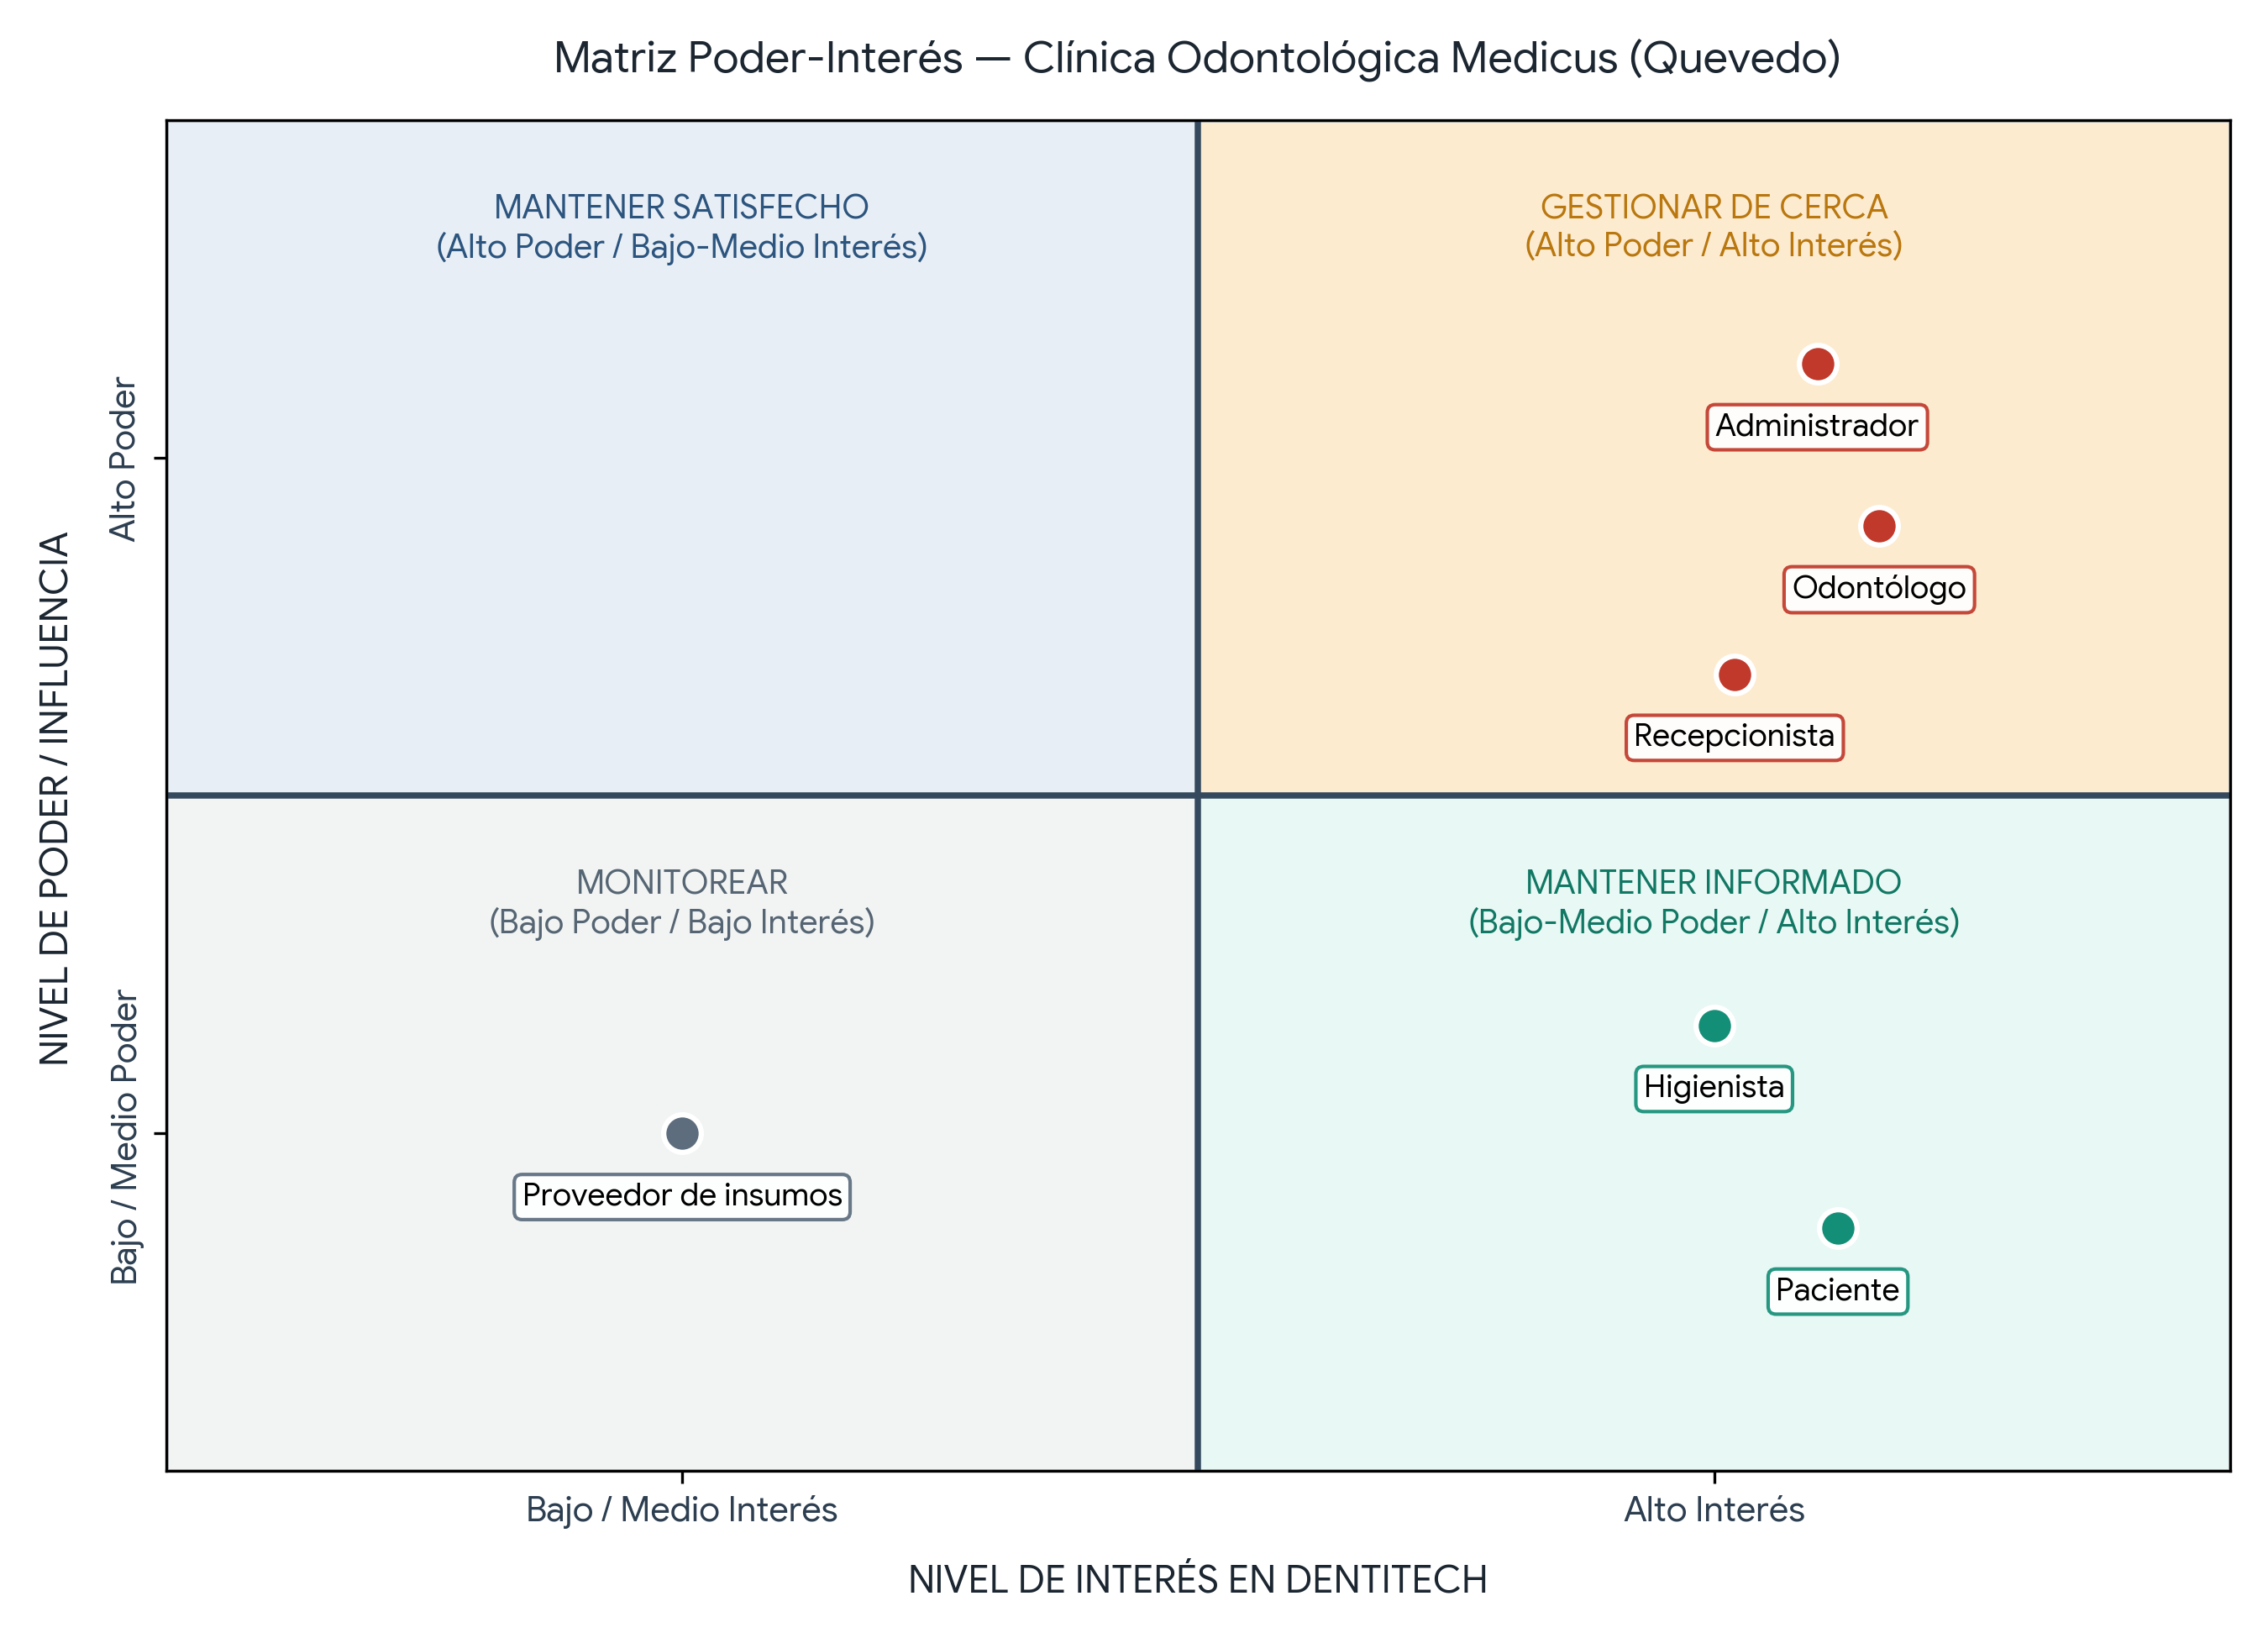
\includegraphics[width=0.88\textwidth]{figuras/matriz_poder_interes.png}
}{
    \fbox{\parbox{0.82\textwidth}{
        \centering
        Imagen pendiente: matriz poder-interés.\\
        Verificar el archivo figuras/matriz\_poder\_interes.png
    }}
}
\caption{Matriz Poder-Interés de las ocho partes interesadas propuestas para DentiTech}
\label{fig:matriz_poder_interes}
\end{figure}

La clasificación de los dos roles complementarios es preliminar y deberá validarse con la clínica. La matriz considera los ocho roles identificados en la caracterización de partes interesadas.

La distribución resultante orienta la estrategia de participación durante la ingeniería de requisitos:

\begin{itemize}
    \item \textbf{Gestionar de cerca (Alto Poder / Alto Interés):} Agrupa al \textbf{Administrador}, al \textbf{Odontólogo} y a la \textbf{Recepcionista}. Estos roles definen las reglas operativas, clínicas y administrativas de la Clínica Odontológica Medicus; su validación continua es indispensable para aprobar los entregables del sistema.

    \item \textbf{Mantener satisfecho (Alto Poder / Bajo-Medio Interés):} No registra actores exclusivos en este cuadrante, dado que los roles con mayor capacidad de decisión en la clínica participan directamente en la operación diaria del sistema.

    \item \textbf{Mantener informado (Bajo-Medio Poder / Alto Interés):} Comprende al \textbf{Higienista}, al \textbf{Paciente}, al \textbf{Asistente dental} y al \textbf{Responsable de contabilidad}. Sus necesidades sobre flujos de preparación clínica, bioseguridad, recordatorios, claridad en presupuestos y seguimiento de cobros se recogen mediante instrumentos focalizados sin sobrecargar las decisiones arquitectónicas.

    \item \textbf{Monitorear (Bajo Poder / Bajo Interés):} Corresponde al \textbf{Proveedor de insumos}, cuya interacción se limita al intercambio estándar de catálogos, lotes, fechas de caducidad y órdenes de reposición.
\end{itemize}

\subsection{Contexto y Límites del Sistema}

Siguiendo los principios de delimitación de contexto establecidos por Pohl \cite{pohl2025} y el programa de estudios IREB \cite{ireb2026}, el diagrama de contexto de la Figura~\ref{fig:diagrama_contexto} establece la frontera entre \textbf{DentiTech} y las ocho entidades externas propuestas de su entorno operativo en la Clínica Odontológica Medicus.

\begin{figure}[htbp]
\centering
\IfFileExists{figuras/diagrama_contexto.png}{
    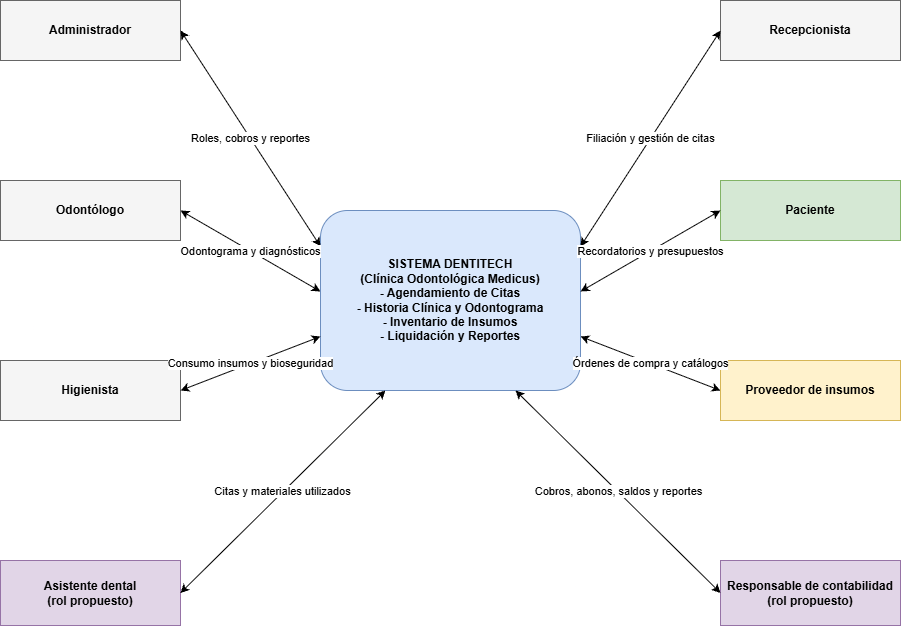
\includegraphics[width=0.95\textwidth]{figuras/diagrama_contexto.png}
}{
    \fbox{\parbox{0.82\textwidth}{
        \centering
        Imagen pendiente: diagrama de contexto.\\
        Verificar el archivo figuras/diagrama\_contexto.png
    }}
}
\caption{Diagrama de contexto del sistema DentiTech y flujos de información con ocho entidades externas}
\label{fig:diagrama_contexto}
\end{figure}

En el modelo de ocho actores, el Asistente dental se relaciona con la consulta de citas y el registro de materiales utilizados, mientras que el Responsable de contabilidad se relaciona con la consulta de cobros, abonos, saldos y reportes. Estas interacciones se proponen para validación.

El sistema central gestiona de manera integrada el agendamiento de citas, la historia clínica odontológica (odontograma, diagnósticos y evoluciones), el control de inventario de insumos y la administración de cobros y reportes. Quedan fuera de la frontera del software los equipos médicos de diagnóstico por imagen (rayos X intraorales) y las plataformas bancarias externas, con las cuales únicamente se registran referencias documentales de resultados o comprobantes de pago.

El diagrama de contexto presenta las interacciones propuestas para los ocho roles, conservando los seis actores originales del modelo elaborado por Landy e incorporando los dos roles complementarios sujetos a validación.

\subsection{Análisis de las Ocho Perspectivas del Contexto}

Para asegurar una comprensión integral del entorno donde operará \textbf{DentiTech} en la Clínica Odontológica Medicus (sector Cooperativa Jet, Quevedo), la Tabla~\ref{tab:ocho_perspectivas} sistematiza el análisis bajo las ocho perspectivas del contexto definidas en el sílabo de la asignatura \cite{ireb2026}.

\begin{table}[htbp]
\centering
\caption{Análisis del entorno operativo de Medicus según ocho perspectivas del contexto}
\label{tab:ocho_perspectivas}
\begingroup
\scriptsize
\setlength{\tabcolsep}{3pt}
\renewcommand{\arraystretch}{1.2}
\begin{tabularx}{\textwidth}{
>{\raggedright\arraybackslash}p{2.25cm}
>{\raggedright\arraybackslash}X
>{\raggedright\arraybackslash}X}
\toprule
\textbf{Perspectiva} &
\textbf{Aspecto evaluado en el dominio odontológico} &
\textbf{Hallazgo en la Clínica Odontológica Medicus}\\
\midrule

1. Negocio / Organizacional &
Estructura jerárquica, flujo de atención al paciente, horarios de consulta y modelo de cobro por procedimientos. &
La clínica opera en el sector Cooperativa Jet de Quevedo brindando atención odontológica bajo esquema de citas programadas y atención por demanda, con cobros por sesión o abonos por tratamiento supervisados por el Administrador.\\
\addlinespace

2. Usuario / Operativa &
Nivel de alfabetización digital del personal (Administrador, Odontólogo, Higienista, Recepcionista) y carga en horas pico. &
El personal clínico y administrativo maneja herramientas ofimáticas básicas; el registro actual de citas y fichas presenta cuellos de botella en horas de mayor afluencia de pacientes.\\
\addlinespace

3. Técnica / Tecnológica &
Equipamiento de cómputo disponible en recepción y consultorios, conectividad a internet y respaldos locales. &
El establecimiento cuenta con estaciones de cómputo en área administrativa y acceso a internet comercial estable, sin un sistema integrado especializado en gestión odontológica.\\
\addlinespace

4. Datos / Información &
Volumen de historias clínicas activas, estructura del odontograma, trazabilidad de abonos e inventario de insumos. &
Las historias clínicas, odontogramas, pagos y movimientos de insumos requieren centralización digital para evitar duplicidad de fichas y facilitar el seguimiento histórico por paciente.\\
\addlinespace

5. Legal / Normativa &
Cumplimiento de la LOPDP del Ecuador \cite{lopdp2021} respecto a datos sensibles de salud, consentimiento informado y normativa sanitaria del MSP. &
La clínica requiere custodia estricta de historias clínicas y consentimientos informados firmados antes de intervenciones invasivas, bajo principios de confidencialidad y control de acceso por rol.\\
\addlinespace

6. Económica / Financiera &
Restricciones presupuestarias para licenciamiento de software, costos de mantenimiento e impacto de insumos caducados. &
Se prioriza una solución sostenible sin costos elevados de licenciamiento recurrente, orientada a reducir pérdidas por caducidad de materiales entregados por el Proveedor de insumos.\\
\addlinespace

7. Cultural / Social &
Hábitos de comunicación de los pacientes de Quevedo (preferencia por mensajería instantánea) y adopción del sistema. &
Los pacientes del sector prefieren confirmaciones y recordatorios ágiles mediante mensajería instantánea, mientras que el equipo clínico demanda interfaces intuitivas de rápida adopción.\\
\addlinespace

8. Ambiental / Física &
Condiciones físicas de los consultorios (iluminación, bioseguridad, uso de guantes durante la consulta) que condicionan la operación. &
La operación clínica del Odontólogo e Higienista exige interfaces de registro rápido con mínima manipulación de periféricos durante la atención y equipos fuera de zonas húmedas.\\
\bottomrule
\end{tabularx}
\endgroup
\end{table}

% FIN DEL APORTE INDIVIDUAL DE LANDY FUERTES

% ===== FIN APORTE =====

% Anderson Alcivar: tabla y correspondencia complementarias.
% Son aportes propios que se conservan; los dos roles adicionales
% siguen pendientes de validacion con Medicus.

% ===== INICIO APORTE: aportes/anderson/02_partes_interesadas_complemento =====
\subsection{Correspondencia con el plan de elicitaci{\'o}n}

Para que las ocho partes interesadas tengan una t{\'e}cnica de elicitaci{\'o}n asignada, la Tabla~\ref{tab:and_correspondencia} relaciona cada rol con su t{\'e}cnica y con el instrumento del directorio \texttt{PFC/E1/instrumentos/}. Los roles 1 a 6 conservan la t{\'e}cnica del plan de elicitaci{\'o}n; los roles 7 y 8 usan la estrategia definida en la Tabla~\ref{tab:and_partes_complementarias}.

\begin{table}[htbp]
\centering
\caption{Correspondencia entre partes interesadas, t{\'e}cnicas e instrumentos}
\label{tab:and_correspondencia}
\small
\begin{tabularx}{\textwidth}{>{\raggedright\arraybackslash}p{0.5cm} >{\raggedright\arraybackslash}p{3.4cm} >{\raggedright\arraybackslash}p{4.2cm} >{\raggedright\arraybackslash}X}
\toprule
\textbf{N.\textsuperscript{o}} & \textbf{Parte interesada} & \textbf{T{\'e}cnica} & \textbf{Instrumento} \\
\midrule
1 & Administrador & Entrevista semiestructurada y revisi{\'o}n documental & Guion 01 (bloque A) y Cuestionario 02 (secci{\'o}n A) \\
2 & Odont{\'o}logo & Entrevista y observaci{\'o}n & Guion 01 (bloque B) y Gu{\'i}a 03 \\
3 & Higienista & Observaci{\'o}n directa y entrevista breve & Gu{\'i}a 03 y Guion 01 (pregunta B-03) \\
4 & Recepcionista & Cuestionario y entrevista & Cuestionario 02 (secci{\'o}n A) y Guion 01 (bloque C) \\
5 & Paciente & Cuestionario breve y observaci{\'o}n & Cuestionario 02 (secciones B y C) \\
6 & Proveedor de insumos & Entrevista breve estructurada & Guion 01 (pregunta C-03) \\
7 & Asistente dental & Entrevista breve y observaci{\'o}n & Gu{\'i}a 03 y Guion 01 (pregunta B-03) \\
8 & Responsable de contabilidad & Entrevista semiestructurada y revisi{\'o}n documental & Guion 01 (preguntas A-02 y A-03) y formatos de cobros y reportes \\
\bottomrule
\end{tabularx}
\end{table}
% ===== FIN APORTE =====


% 4. PLAN DE ELICITACION E INSTRUMENTOS (Aporte de Frixon)
\section{Plan de Elicitaci{\'o}n de Requisitos}
El levantamiento de requisitos para \textit{DentiTech} en la \textbf{Cl{\'i}nica Odontol{\'o}gica Medicus} (Cooperativa Jet, Quevedo) se planifica considerando la naturaleza de cada rol, el tipo de conocimiento involucrado (t{\'a}cito, expl{\'i}cito, procedimental o normativo) y la disponibilidad operativa de la cl{\'i}nica \cite{iso29148, pohl2025}.
\subsection{Selecci{\'o}n de T{\'e}cnicas por Rol de Parte Interesada}
A continuaci{\'o}n se detalla la t{\'e}cnica de elicitaci{\'o}n asignada a cada uno de los ocho roles propuestos para el sistema \textit{DentiTech}, justificando su pertinencia seg{\'u}n el conocimiento requerido y la fuente de informaci{\'o}n.
\begin{table}[htbp]
\centering
\caption{Plan de elicitaci{\'o}n por rol para la Cl{\'i}nica Odontol{\'o}gica Medicus}
\label{tab:plan_elicitacion_medicus}
\begin{adjustbox}{max width=\textwidth}
\begin{tabularx}{\textwidth}{>{\raggedright\arraybackslash}p{2.7cm} >{\raggedright\arraybackslash}p{2.4cm} >{\raggedright\arraybackslash}p{2.6cm} >{\raggedright\arraybackslash}p{2.5cm} >{\raggedright\arraybackslash}X}
\toprule
\textbf{Rol} & \textbf{Tipo de Conocimiento} & \textbf{Fuente} & \textbf{T{\'e}cnica} & \textbf{Justificaci{\'o}n} \\
\midrule
Administrador & Estrat{\'e}gico, operativo y t{\'e}cnico & Gesti{\'o}n general, pol{\'i}ticas, cobros e infraestructura & Entrevista semiestructurada y revisi{\'o}n documental & Permite capturar reglas de negocio, flujos administrativos, presupuestos/pagos, respaldos y controles de acceso en Medicus. \\
\addlinespace
Odont{\'o}logo & T{\'a}cito y cl{\'i}nico & Atenci{\'o}n en sill{\'o}n, diagn{\'o}stico y odontograma & Entrevista y observaci{\'o}n & Combina el criterio cl{\'i}nico y de tratamiento con el flujo real de consulta sin interrumpir la atenci{\'o}n. \\
\addlinespace
Higienista & Procedimental y cl{\'i}nico & Preparaci{\'o}n de gabinete, profilaxis e insumos & Observaci{\'o}n directa y entrevista breve & Registra rutinas de apoyo cl{\'i}nico, esterilizaci{\'o}n, preparaci{\'o}n de instrumental y uso de materiales. \\
\addlinespace
Recepcionista & Operativo y expl{\'i}cito & Agenda, admisi{\'o}n y atenci{\'o}n inicial & Cuestionario y entrevista & Facilita cuantificar citas, reprogramaciones, motivos de consulta y cuellos de botella en recepci{\'o}n. \\
\addlinespace
Paciente & Experiencial y t{\'a}cito & Reserva, sala de espera y consulta & Cuestionario breve y observaci{\'o}n & Identifica fricciones al agendar, tiempos de espera y claridad en la comunicaci{\'o}n y seguimiento. \\
\addlinespace
Proveedor de insumos & Externo y expl{\'i}cito & Pedidos, entregas y cat{\'a}logos & Entrevista breve estructurada & Clarifica plazos de reposici{\'o}n, presentaciones de insumos odontol{\'o}gicos y condiciones de suministro. \\
\addlinespace
Asistente dental & Procedimental y cl{\'i}nico & Preparaci{\'o}n del consultorio y uso de materiales & Entrevista breve y observaci{\'o}n & Permite identificar tareas de apoyo y necesidades de registro de insumos; rol propuesto pendiente de validaci{\'o}n con Medicus. \\
\addlinespace
Responsable de contabilidad & Administrativo y expl{\'i}cito & Cobros, abonos, saldos y reportes & Entrevista semiestructurada y revisi{\'o}n documental & Permite precisar reportes y controles de pagos; rol propuesto pendiente de validaci{\'o}n con Medicus. \\
\bottomrule
\end{tabularx}
\end{adjustbox}
\end{table}
\subsection{Cronograma de Sesiones y Artefactos Esperados}

Las sesiones de levantamiento se programan en coordinaci{\'o}n con la direcci{\'o}n de \textit{Medicus} para aprovechar ventanas de menor afluencia y contar con instrumentos estructurados que agilicen cada encuentro.
\begin{table}[htbp]
\centering
\caption{Cronograma de sesiones de elicitaci{\'o}n y artefactos esperados}
\label{tab:cronograma_elicitacion}
\begin{adjustbox}{max width=\textwidth}
\begin{tabularx}{\textwidth}{>{\raggedright\arraybackslash}p{2.2cm} >{\raggedright\arraybackslash}p{3.2cm} >{\raggedright\arraybackslash}p{2.6cm} >{\raggedright\arraybackslash}X}
\toprule
\textbf{Sesi{\'o}n / Fase} & \textbf{Roles Convocados} & \textbf{Instrumento} & \textbf{Artefactos Esperados} \\
\midrule
Sesi{\'o}n 1 (Sem. 5) & Administrador y Recepcionista & Guion de entrevista y cuestionario & Acta de sesi{\'o}n, cuestionarios diligenciados y registro de reglas operativas, agenda y cobros. \\
\addlinespace
Sesi{\'o}n 2 (Sem. 6) & Odont{\'o}logo e Higienista & Gu{\'i}a de observaci{\'o}n y entrevista & Ficha de observaci{\'o}n anonimizada, notas de flujo cl{\'i}nico y observaciones de odontograma e insumos. \\
\addlinespace
Sesi{\'o}n 3 (Sem. 6) & Pacientes y Proveedor de insumos & Cuestionario breve y entrevista & Consolidado anonimizado de respuestas de pacientes y notas sobre tiempos y modalidades de abastecimiento. \\
\bottomrule
\end{tabularx}
\end{adjustbox}
\end{table}

Los dos roles complementarios se incorporan de manera provisional a las sesiones de levantamiento, sujetos a confirmaci{\'o}n de su existencia y disponibilidad por parte de Medicus.

Los instrumentos previstos para estas actividades se organizarán en el directorio \texttt{PFC/E1/instrumentos/} bajo los nombres \texttt{01\_guion\_entrevista.pdf}, \texttt{02\_cuestionario.pdf} y \texttt{03\_guia\_observacion.pdf}.

% 5. ETICA Y PROTECCION DE DATOS PERSONALES (Aporte de Frixon)
El levantamiento de informaci{\'o}n en la \textbf{Cl{\'i}nica Odontol{\'o}gica Medicus} involucra procesos cl{\'i}nicos, administrativos y de atenci{\'o}n a pacientes, por lo que su ejecuci{\'o}n se ajusta a los principios {\'e}ticos de la investigaci{\'o}n acad{\'e}mica y a la Ley Org{\'a}nica de Protecci{\'o}n de Datos Personales (\textbf{LOPDP}) del Ecuador \cite{lopdp2021, reglamento_lopdp2023}.

\subsection{Protocolo de Anonimizaci{\'o}n}

Antes de incorporar cualquier evidencia al repositorio o a los documentos del proyecto \textit{DentiTech}, se aplica un procedimiento estricto de anonimizaci{\'o}n:
\begin{itemize}
    \item \textbf{Eliminaci{\'o}n de identificadores directos:} Se omiten nombres completos, n{\'u}meros de c{\'e}dula, tel{\'e}fonos, correos electr{\'o}nicos personales, direcciones domiciliarias, c{\'o}digos de historia cl{\'i}nica y fotograf{\'i}as o grabaciones que permitan reconocer a personas.
    \item \textbf{Seudonimizaci{\'o}n por rol y c{\'o}digo:} Cada participante se identifica mediante un c{\'o}digo funcional y correlativo (por ejemplo, \texttt{MED-ADM-01}, \texttt{MED-ODO-01}, \texttt{MED-HIG-01}, \texttt{MED-REC-01}, \texttt{MED-PAC-01}, \texttt{MED-PRV-01}).
    \item \textbf{Revisi{\'o}n previa a cada commit:} Antes de subir archivos a GitHub, el responsable verifica que no existan datos personales ni documentos firmados en las carpetas del repositorio p{\'u}blico.
\end{itemize}
\subsection{Custodia de Evidencias y Cumplimiento LOPDP}

Para garantizar la confidencialidad, integridad y trazabilidad de la informaci{\'o}n recabada en \textit{Medicus}:
\begin{itemize}
    \item \textbf{Almacenamiento de informaci{\'o}n sensible:} Ning{\'u}n dato personal, audio, video, captura con datos reales ni consentimiento firmado se sube al repositorio p{\'u}blico de GitHub. Dichos respaldos, cuando correspondan, se conservan exclusivamente en la carpeta privada institucional \texttt{@uteq.edu.ec} compartida con el docente.
    \item \textbf{Trazabilidad mediante hash SHA-256:} Los archivos sensibles resguardados en el entorno privado institucional se registran mediante su huella \texttt{SHA-256} en el manifiesto del proyecto para verificar su integridad sin exponer su contenido.
    \item \textbf{Derechos de los titulares:} Los participantes son informados sobre el car{\'a}cter acad{\'e}mico del levantamiento y sobre sus derechos de acceso, rectificaci{\'o}n, eliminaci{\'o}n y oposici{\'o}n previstos en la LOPDP.
\end{itemize}
\subsection{Consentimiento Informado}

Toda entrevista, cuestionario u observaci{\'o}n en la cl{\'i}nica se realiza previa entrega y explicaci{\'o}n del formato de consentimiento informado, incluido en blanco como \texttt{PFC/E1/instrumentos/04\_consentimiento\_informado.pdf}. En dicho documento se especifica el objetivo del proyecto \textit{DentiTech}, el car{\'a}cter libre y voluntario de la participaci{\'o}n, la ausencia de impacto cl{\'i}nico en la atenci{\'o}n del paciente y las condiciones de confidencialidad y protecci{\'o}n de datos.





% 6. GESTION DEL PROYECTO Y DECLARACION DE USO DE IA (Aporte de Kevin)
\section{Gesti{\'o}n del Proyecto}

La gesti{\'o}n del Proyecto Fin de Curso (PFC) correspondiente al sistema \textit{DentiTech} para la cl{\'i}nica odontol{\'o}gica \textit{Medicus} (ubicada en el sector Cooperativa Jet, cant{\'o}n Quevedo, provincia de Los R{\'i}os) se estructura bajo los principios de direcci{\'o}n de proyectos establecidos en la gu{\'i}a PMBOK \cite{pmbok2021}. Esta planificaci{\'o}n garantiza la trazabilidad de los entregables, el cumplimiento de los hitos acad{\'e}micos de la asignatura Ingenier{\'i}a de Requerimientos (ISR-401) y la coordinaci{\'o}n efectiva con la organizaci{\'o}n cliente.

\subsection{Roles y Responsabilidades del Equipo}

El equipo de trabajo est{\'a} conformado por cuatro estudiantes de cuarto nivel de la Carrera de Software de la Universidad T{\'e}cnica Estatal de Quevedo (UTEQ). Con el prop{\'o}sito de asegurar una distribuci{\'o}n equitativa y verificable mediante el control de versiones en GitHub, se asignaron los roles detallados en la Tabla~\ref{tab:roles_equipo}.

\begin{table}[htbp]
\centering
\caption{Distribuci{\'o}n de roles y responsabilidades del equipo de proyecto}
\label{tab:roles_equipo}
\begin{adjustbox}{max width=\textwidth}
\begin{tabularx}{\textwidth}{>{\raggedright\arraybackslash}p{4.2cm} >{\raggedright\arraybackslash}p{3.8cm} >{\raggedright\arraybackslash}X}
\toprule
\textbf{Integrante} & \textbf{Rol Asignado} & \textbf{Responsabilidades Principales} \\
\midrule
Alc{\'i}var V{\'e}lez Anderson Adonis & Analista de Negocio y Partes Interesadas & Levantamiento de informaci{\'o}n institucional de Medicus, definici{\'o}n de visi{\'o}n, objetivos medibles, l{\'i}mites de alcance y caracterizaci{\'o}n de partes interesadas. \\
\addlinespace
Contreras Ch{\'a}vez Kevin Germ{\'a}n & Integrador LaTeX, Arquitectura del Repositorio y Gesti{\'o}n & Administraci{\'o}n del repositorio GitHub, estructuraci{\'o}n documental en LaTeX, gesti{\'o}n bibliogr{\'a}fica IEEE, cronograma, plan de comunicaci{\'o}n y matriz de riesgos. \\
\addlinespace
Fuertes Calvo Landy Lorena & Arquitecta de Contexto y Modelado Visual & Elaboraci{\'o}n del diagrama de contexto editable, an{\'a}lisis de las ocho perspectivas del s{\'i}labo y construcci{\'o}n de la matriz poder-inter{\'e}s. \\
\addlinespace
Mor{\'a}n Pilaguano Frixon Fernando & Especialista en Elicitaci{\'o}n y {\'E}tica de Datos & Dise{\~n}o del plan de elicitaci{\'o}n, elaboraci{\'o}n de instrumentos (entrevista, cuestionario y observaci{\'o}n), protocolo de consentimiento informado y manifiesto de evidencias. \\
\bottomrule
\end{tabularx}
\end{adjustbox}
\end{table}

\subsection{Cronograma General hasta la Semana 17}

El desarrollo de \textit{DentiTech} abarca desde la identificaci{\'o}n inicial del problema en la Semana 4 hasta la validaci{\'o}n y entrega final en la Semana 17 del per{\'i}odo acad{\'e}mico SPA 2026-2027. La Tabla~\ref{tab:cronograma_pfc} resume las fases, actividades clave y productos verificables planificados.

\begin{table}[htbp]
\centering
\caption{Cronograma de actividades del PFC DentiTech (Semanas 4 a 17)}
\label{tab:cronograma_pfc}
\begin{adjustbox}{max width=\textwidth}
\begin{tabularx}{\textwidth}{>{\centering\arraybackslash}p{2.2cm} >{\raggedright\arraybackslash}p{4.2cm} >{\raggedright\arraybackslash}X >{\raggedright\arraybackslash}p{3.3cm}}
\toprule
\textbf{Semanas} & \textbf{Fase del Proyecto} & \textbf{Actividades Principales} & \textbf{Entregable / Hito} \\
\midrule
Semana 4 & Inicio, Visi{\'o}n y Planificaci{\'o}n (E1) & Formalizaci{\'o}n de contacto con Medicus, definici{\'o}n de alcance, matriz de interesados, contexto e instrumentos de elicitaci{\'o}n. & Informe E1 en LaTeX y repositorio base. \\
\addlinespace
Semanas 5--6 & Ejecuci{\'o}n de Elicitaci{\'o}n & Aplicaci{\'o}n de entrevistas, cuestionarios y observaci{\'o}n directa en Medicus; registro y anonimizaci{\'o}n de evidencias. & Actas, transcripciones y matriz de hallazgos. \\
\addlinespace
Semanas 7--8 & An{\'a}lisis y Clasificaci{\'o}n & Depuraci{\'o}n de necesidades, resoluci{\'o}n de conflictos entre roles y clasificaci{\'o}n de requisitos funcionales y no funcionales \cite{iso29148}. & Cat{\'a}logo preliminar de requisitos (E2). \\
\addlinespace
Semanas 9--11 & Modelado de Requisitos & Construcci{\'o}n de diagramas de casos de uso, modelos de procesos de atenci{\'o}n odontol{\'o}gica, modelos de datos y m{\'a}quinas de estado. & Modelos UML y diccionario de datos. \\
\addlinespace
Semanas 12--14 & Especificaci{\'o}n ERS y Prototipado & Redacci{\'o}n de la Especificaci{\'o}n de Requisitos de Software (ERS) seg{\'u}n ISO/IEC/IEEE 29148 y dise{\~n}o de prototipos de interfaz. & Documento ERS v1.0 y maquetas funcionales. \\
\addlinespace
Semanas 15--16 & Verificaci{\'o}n y Validaci{\'o}n & Inspecci{\'o}n t{\'e}cnica de calidad, matriz de trazabilidad bidireccional y sesi{\'o}n de validaci{\'o}n con el personal de Medicus. & Acta de validaci{\'o}n y ERS ajustada. \\
\addlinespace
Semana 17 & Cierre y Sustentaci{\'o}n Final & Integraci{\'o}n final del repositorio, verificaci{\'o}n de reproducibilidad documental y sustentaci{\'o}n ante el tribunal docente. & Entrega final PFC y defensa t{\'e}cnica. \\
\bottomrule
\end{tabularx}
\end{adjustbox}
\end{table}

\subsection{Plan de Comunicaci{\'o}n con la Organizaci{\'o}n}

Para evitar interrupciones en la jornada cl{\'i}nica de \textit{Medicus} y mantener un canal formal de coordinaci{\'o}n, se establece el protocolo de comunicaci{\'o}n descrito en la Tabla~\ref{tab:plan_comunicacion}. Toda evidencia recabada se resguarda conforme a la Ley Org{\'a}nica de Protecci{\'o}n de Datos Personales \cite{lopdp2021, reglamento_lopdp2023}.

\begin{table}[htbp]
\centering
\caption{Plan de comunicaci{\'o}n con la cl{\'i}nica odontol{\'o}gica Medicus}
\label{tab:plan_comunicacion}
\begin{adjustbox}{max width=\textwidth}
\begin{tabularx}{\textwidth}{>{\raggedright\arraybackslash}p{3.2cm} >{\raggedright\arraybackslash}p{3.0cm} >{\raggedright\arraybackslash}p{2.6cm} >{\raggedright\arraybackslash}X}
\toprule
\textbf{Instancia} & \textbf{Participantes} & \textbf{Canal y Frecuencia} & \textbf{Prop{\'o}sito y Registro} \\
\midrule
Formalizaci{\'o}n y aval institucional & Responsable de Medicus y Analista de Negocio & Presencial / Carta f{\'i}sica (Inicio PFC) & Aprobaci{\'o}n del estudio y firma de carta de aceptaci{\'o}n institucional. \\
\addlinespace
Sesiones de elicitaci{\'o}n y observaci{\'o}n & Personal cl{\'i}nico, recepci{\'o}n y Especialista en Elicitaci{\'o}n & Presencial en Medicus (Semanas 5--6) & Levantamiento de flujos de citas, historias cl{\'i}nicas y cobros previa firma de consentimiento. \\
\addlinespace
Validaci{\'o}n de modelos y prototipos & Direcci{\'o}n de Medicus y equipo desarrollador & Presencial / Videollamada (Semanas 11 y 15) & Revisi{\'o}n de alcance, reglas de negocio y prototipos de interfaz de \textit{DentiTech}. \\
\addlinespace
Consultas operativas r{\'a}pidas & Enlace operativo de Medicus e Integrador & Mensajer{\'i}a institucional (Seg{\'u}n demanda) & Confirmaci{\'o}n de horarios de visita y aclaraci{\'o}n puntual de formatos cl{\'i}nicos. \\
\bottomrule
\end{tabularx}
\end{adjustbox}
\end{table}

\subsection{Registro de Riesgos del Proyecto}

Se identificaron seis riesgos principales asociados tanto a la operaci{\'o}n diaria de \textit{Medicus} en Quevedo como a la ejecuci{\'o}n t{\'e}cnica del equipo, junto con sus estrategias de mitigaci{\'o}n (Tabla~\ref{tab:registro_riesgos}).

\begin{table}[htbp]
\centering
\caption{Registro y plan de mitigaci{\'o}n de riesgos del proyecto DentiTech}
\label{tab:registro_riesgos}
\begin{adjustbox}{max width=\textwidth}
\begin{tabularx}{\textwidth}{>{\centering\arraybackslash}p{1.2cm} >{\raggedright\arraybackslash}p{3.8cm} >{\centering\arraybackslash}p{2.0cm} >{\centering\arraybackslash}p{1.8cm} >{\raggedright\arraybackslash}X}
\toprule
\textbf{ID} & \textbf{Descripci{\'o}n del Riesgo} & \textbf{Probabilidad} & \textbf{Impacto} & \textbf{Estrategia de Mitigaci{\'o}n} \\
\midrule
R-01 & Demora en la formalizaci{\'o}n escrita de la carta de aceptaci{\'o}n por disponibilidad del responsable de Medicus. & Alta & Alto & Gestionar la firma presencial mediante el enlace interno al inicio de la Semana 5 y documentar el primer contacto en el manifiesto. \\
\addlinespace
R-02 & Interrupci{\'o}n de entrevistas por atenci{\'o}n de urgencias odontol{\'o}gicas durante la jornada laboral. & Alta & Medio & Agendar bloques cortos de 20 minutos en horarios de menor flujo y emplear cuestionarios estructurados como respaldo. \\
\addlinespace
R-03 & Ambig{\"u}edad en reglas de presupuestos, abonos parciales y odontogramas entre especialistas. & Media & Alto & Contrastar los registros f{\'i}sicos actuales de Medicus mediante observaci{\'o}n directa y validar las reglas con el odont{\'o}logo principal \cite{pohl2025}. \\
\addlinespace
R-04 & Exposici{\'o}n accidental de datos sensibles de pacientes en evidencias o capturas del repositorio p{\'u}blico. & Baja & Muy Alto & Aplicar anonimizaci{\'o}n estricta antes de exportar archivos y almacenar documentos originales {\'u}nicamente en la carpeta privada institucional \cite{lopdp2021}. \\
\addlinespace
R-05 & Desviaci{\'o}n del alcance (\textit{scope creep}) por solicitudes de m{\'o}dulos contables o tributarios complejos no previstos. & Media & Alto & Mantener una matriz de trazabilidad frente a los l{\'i}mites definidos en E1 y registrar nuevas peticiones como mejoras futuras \cite{wiegers2013}. \\
\addlinespace
R-06 & Conflictos de integraci{\'o}n en LaTeX o entregas tard{\'i}as en el repositorio GitHub. & Media & Medio & Estandarizar subcarpetas por integrante, realizar integraciones parciales tempranas y validar la compilaci{\'o}n en Overleaf. \\
\bottomrule
\end{tabularx}
\end{adjustbox}
\end{table}

\section{Declaraci{\'o}n de Uso de Inteligencia Artificial}

En cumplimiento de las normas de integridad acad{\'e}mica de la asignatura, se declara el uso de herramientas de inteligencia artificial generativa exclusivamente como apoyo t{\'e}cnico y editorial durante la elaboraci{\'o}n de este informe:

\begin{itemize}
    \item \textbf{Herramientas utilizadas:} Google Gemini (seg{\'u}n la declaraci{\'o}n original del equipo) y ChatGPT de OpenAI (apoyo posterior a la integraci{\'o}n documental y correcciones LaTeX).
    \item \textbf{Prop{\'o}sito del uso:} Asistencia en la estructuraci{\'o}n de plantillas y tablas en lenguaje LaTeX, configuraci{\'o}n de comandos de control de versiones en Git y revisi{\'o}n ortogr{\'a}fica y de estilo t{\'e}cnico en espa{\~n}ol.
    \item \textbf{Mecanismo de verificaci{\'o}n y autor{\'i}a:} El equipo defini{\'o} de forma aut{\'o}noma el caso de estudio de la cl{\'i}nica odontol{\'o}gica \textit{Medicus} en Quevedo, el alcance del sistema \textit{DentiTech}, los roles, el cronograma y los instrumentos de elicitaci{\'o}n. Los fragmentos de c{\'o}digo LaTeX sugeridos requieren revisi{\'o}n del equipo, compilaci{\'o}n y contraste con las fuentes bibliogr{\'a}ficas originales en formato IEEE \cite{iso29148, pohl2025, ireb2026}.
\end{itemize}

\bibliographystyle{IEEEtran}
\bibliography{referencias}

\end{document}
